\documentclass[../src/handouts/main.tex]{subfiles}
% note that the CWD (.) above is the output directory of pdflatex
% (<repo-root-dir>/build)

% path that contains required images
\graphicspath{ {../src/handouts/figures/} }

% This document depends on the other sections, which provides
% the following references (in the order of references in this section):
%   prop:con-degree-sum
%   cor:con-odd-degree
%   rem:con-iff
%   princ:intro-pigeonhole
% As a result, compiling only this document gives undefined references.

% prevent \recall theorems outside this section
% if this section is compiled solely
\def\sectionprefix{matching}%

\begin{document}

% TODO: use TikZ to replace almost all figures

\section{Matchings and Factors}

\subsection{Chinese Postman Problem}

This is 2.3.9. Application in the textbook.

\begin{enumerate}
  \item A mail carrier must traverse all edges in a road network, starting and ending at the post office.
  \item The edges have nonnegative weights representing distance, time or fuel cost.
  \item \textbf{We seek a closed walk of minimum total length that uses all the edges.}
  \item \textbf{Key Points}: If every vertex is even, then the graph is Eulerian and the answer is the sum of the edge weights. Otherwise, we must repeat edges.
  \item If there are only two odd vertices, then use Dijkstra's algorithm to find the shortest path between them.
  \item If there are $2 k$ odd vertices (\cref{prop:con-degree-sum,cor:con-odd-degree}), then
    \begin{enumerate}
      \item Use Dijkstra's algorithm to find the shortest paths connecting each pair of odd vertices.
      \item Construct a helper graph with these lengths as weights on the edges of $K_{2 k}$ (a complete graph with $2 k$ vertices).
      \item Solve the weighted version of the \textbf{maximum matching problem} on $K_{2 k}$. In a matching of two odd edges, they share no common vertex. The maximum matchings means the most number of matchings. In this case, we need $k$ pairs of edges such that the sum of weights of these $k$ pairs is minimum (required by the problem).
    \end{enumerate}
\end{enumerate}

\begin{figure}[htbp]
  \centering
  \begin{subfigure}[t]{.3\textwidth}
    \centering
    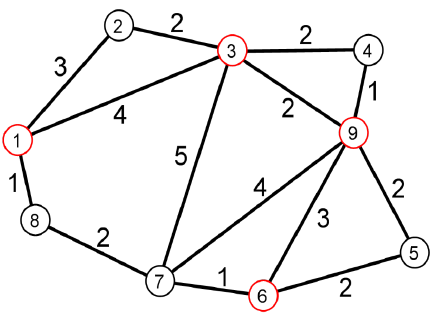
\includegraphics[width=\textwidth]{mat-chinese-postman-question}
    \caption{The graph from the problem.}
    \label{fig:mat-chinese-postman-question}
  \end{subfigure}
  \hspace{.025\textwidth}
  \begin{subfigure}[t]{.3\textwidth}
    \centering
    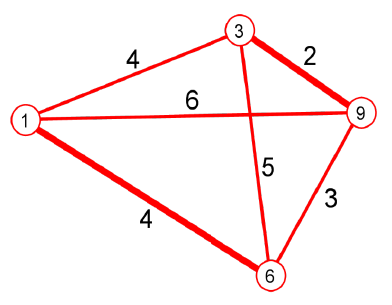
\includegraphics[width=\textwidth]{mat-chinese-postman-helper}
    \caption{In the helper graph.}
    \label{fig:mat-chinese-postman-helper}
  \end{subfigure}
  \hspace{.025\textwidth}
  \begin{subfigure}[t]{.3\textwidth}
    \centering
    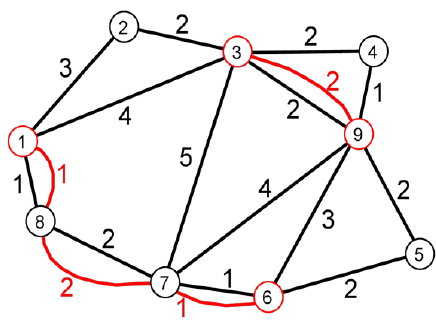
\includegraphics[width=\textwidth]{mat-chinese-postman-with-matchings}
    \caption{Merge the matchings back to the original graph with the edges required to construct the shortest paths of these edges in the helper graph. Now we have only even vertices, so the cost the sum of weights.}
    \label{fig:mat-chinese-postman-helper-with-matchings}
  \end{subfigure}
\end{figure}

\subsection{Matchings and Covers}

\begin{definition}{}{mat-matching}
  (3.1.1. Definition in text)
  A \textbf{matching} in a graph $G$ is a set of non-loop \textbf{edges} with no shared endpoints.

  The vertices incident to the edges of a matching $M$ are \textbf{saturated} (infected) by $M$; the others are \textbf{unsaturated}. We say a vertex is $M$-saturated or $M$-unsaturated.

  A \textbf{perfect matching} in a graph is a matching that saturates every vertex.
\end{definition}

\begin{figure}[htbp]
  \centering
  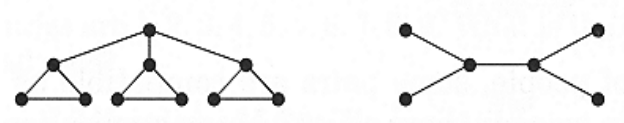
\includegraphics[width=.4\textwidth]{mat-perfect-matching}
  \caption{The two graphs above have no perfect matching.}
  \label{fig:mat-perfect-matching}
\end{figure}

\begin{definition}{}{mat-maximum-matching}
  (3.1.4. Definition in text)
  A \textbf{maximal matching} in a graph is a matching that cannot be enlarged by adding an edge. A \textbf{maximum matching} is a matching of maximum size among all matchings in the graph.
\end{definition}

In \cref{def:mat-maximum-matching}, note that we say "a" maximum matching because there may be multiple maximum matchings. For example, there are two maximum combinations of couples for 2 boys and 2 girls.

\begin{example}{Maximal $\neq$ maximum}{mat-maximal-matching}
  (3.1.5. Example in text)
  The smallest graph having a maximal matching that is not a maximum matching is $P_4$. If we take the middle edge, then we can add no other, but the two end edges form a larger matching. Below we show this phenomenon in $P_4$ and in $P_6$. Replacing the bold edges by the solid edges yields a larger matching. This gives us a way to look for larger matchings.

  \centering
  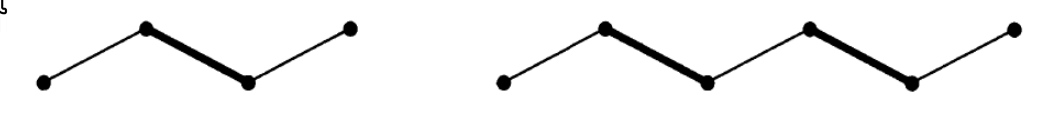
\includegraphics[width=.7\textwidth]{mat-maximal-matching}
\end{example}

If there is a perfect matching, such matching is a maximum matching. However, a maximum matching doesn't imply a perfect matching.

\begin{definition}{}{mat-alternating}
  (3.1.6. Definition in text)
  Given a matching $M$, an $M$\textbf{-alternating path} is a path that alternates between edges in $M$ and edges not in $M$. An $M$-alternating path whose endpoints are unsaturated by $M$ is an $M$\textbf{-augmenting path}.
\end{definition}

For example of \cref{def:mat-alternating}, the two paths in \cref{ex:mat-maximal-matching} are both alternating paths and augmenting paths. However, if we use any maximum matching of the two paths, such paths will only be alternating paths.

Note that an augmenting path is an alternating path.

\begin{definition}{}{mat-symmetric-difference}
  (3.1.6. Definition in text)
  Symmetric difference on matchings (set of edges): For two matchings $M$ and $M'$,
  \[
    M \smalltriangleup M' = \left(M - M'\right) \cup \left(M' - M\right)
  \]
\end{definition}

\begin{example}{}{mat-symmetric-difference}
  (3.1.8. Example in text)
  In the graph below, $M$ is the matching with five solid edges, $M'$ is the one with six bold edges, and the dashed edges belong to neither $M$ nor $M'$.

  \begin{center}
    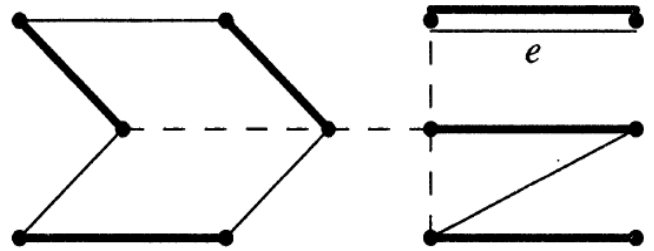
\includegraphics[width=.4\textwidth]{mat-symmetric-difference}
  \end{center}

  The two matchings have one common edge $e$; it is not in their symmetric difference.

  The edges of $M \smalltriangleup M'$ form a cycle of length 6 on the left and a path of length 3 on the bottom right.
\end{example}

\begin{lemma}{}{mat-component-in-symmetric-difference}
  (3.1.9. Lemma in text)
  Every component of the symmetric difference of two matchings is a path or an even cycle.
\end{lemma}

\textbf{Proof} of \cref{lem:mat-component-in-symmetric-difference}:
\begin{enumerate}
  \item Idea: Each vertex degree in a path or a cycle will be not be larger than 2. ($\Delta(P) \leq 2$ and $\Delta(C) \leq 2$.)
  \item Let $M$ and $M'$ be matchings, and let $F = M \smalltriangleup M'$.
  \item Since $M$ and $M'$ are matchings, every vertex has at most one incident edge from each of them. Thus $F$ has at most two edges at each vertex. There is never a condition for the left graph in \cref{fig:mat-component-in-symmetric-difference} to exist.
  \item Since $\Delta(F) \leq 2$, every component of $F$ is a path or a cycle. Furthermore, every path or cycle in $F$ alternates between edges of $M - M'$ and edges of $M' - M$.
  \item Thus each cycle has even length, with an equal number of edges from $M$ and from $M'$.
\end{enumerate}

\begin{figure}[htbp]
  \centering
  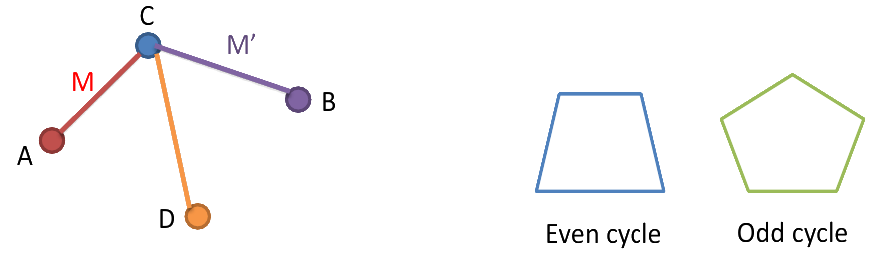
\includegraphics[width=.8\textwidth]{mat-component-in-symmetric-difference}
  \caption{Graphs for illustration of \cref{lem:mat-component-in-symmetric-difference}.}
  \label{fig:mat-component-in-symmetric-difference}
\end{figure}

\begin{theorem}{}{mat-maximum-matching-augmenting-path}
  (3.1.10. Theorem in text) (Berge [1957])
  A matching $M$ in a graph $G$ is a maximum matching in $G$ if and only if $G$ has no $M$-augmenting path.
\end{theorem}

\begin{figure}[htbp]
  \centering
  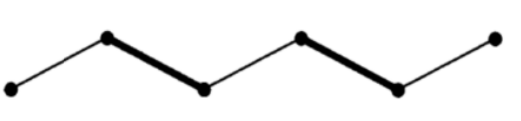
\includegraphics[width=.3\textwidth]{mat-maximum-matching-augmenting-path}
  \caption{An $M$-augmenting path, where $M$ is bold edges.}
  \label{fig:mat-maximum-matching-augmenting-path}
\end{figure}

\textbf{Proof} of \cref{thm:mat-maximum-matching-augmenting-path}:
\begin{enumerate}
  \item Since proving $P \iff Q$ requires more efforts, we prove it with the contrapositive method (\cref{rem:con-iff}). That is, to prove $\neg P \iff \neg Q$, or to prove

    "There is a matching in a graph $G$ larger than $M$ iff. there is an $M$-augmenting path in $G$".

    Note that the two endpoints of $M$ are not in the $M$-augmenting path, but may be in the other matching.
  \item We choose the easiest direction to prove first. That is, to prove $\neg Q \implies \neg P$:
    \begin{enumerate}
      \item In \cref{fig:mat-maximum-matching-augmenting-path}, it is an $M$-augmenting path, where $M$ is the bold edges.
      \item In \cref{fig:mat-maximum-matching-augmenting-path}, $M'$ with solid edges is a larger matching than $M$.
    \end{enumerate}

  \item The most difficult direction is as follows:
    \begin{enumerate}
      \item We have observed that an $M$-augmenting path can be used to produce a matching larger than $M$.
      \item For the converse, let $M'$ be a matching in $G$ larger than $M$; we construct an $M$-augmenting path. Let $F = M \smalltriangleup M'$.
      \item By \cref{lem:mat-component-in-symmetric-difference}, $F$ consists of paths and even cycles; the cycles have the same number of edges from $M$ and $M'$. Since $\abs{M'} > \abs{M}$, $F$ must have a component with more edges of $M'$ than of $M$.
      \item Such a component can only be a path that starts and ends with an edge of $M'$; thus it is an $M$-augmenting path in $G$.
    \end{enumerate}
\end{enumerate}

\begin{theorem}{Hall's Mathcing Theorem}{mat-hall-matching}
  (3.1.11. Theorem in text) (Hall's Theorem-P. Hall [1935])
  An $X, Y$-bigraph $G$ has a matching that saturates $X$ if and only if "$\abs{N(S)} \geq \abs{S}$ for all $S \subseteq X$" (Hall's matching condition). $N(S)$ means the neighbors of $S$, and $N(S) \subseteq Y$.
\end{theorem}

\textbf{Proof} of \cref{thm:mat-hall-matching}: To prove $P \implies Q$:

\begin{enumerate}
  \item We want to prove it by contradiction and the Pigeonhole Principle (\cref{princ:intro-pigeonhole}).
  \item For an $X, Y$-bigraph $G$, in which there is a matching $M$ that saturates $X$.
  \item Let $S \subseteq X$. Since $M$ exists and saturates $X$, there must be a matching $M'$ to saturate $S$.
  \item Assume that $\abs{N(S)} < \abs{S}$. By the Pigeonhole Principle, there is at least one common node shared by some edges in $M'$ to make $M'$ not a matching.
  \item As a result, the assumption is wrong.
  \item See \cref{fig:mat-hall-matching} for the illustration of $S$ and $N(S)$.
\end{enumerate}

\begin{figure}[htbp]
  \centering
  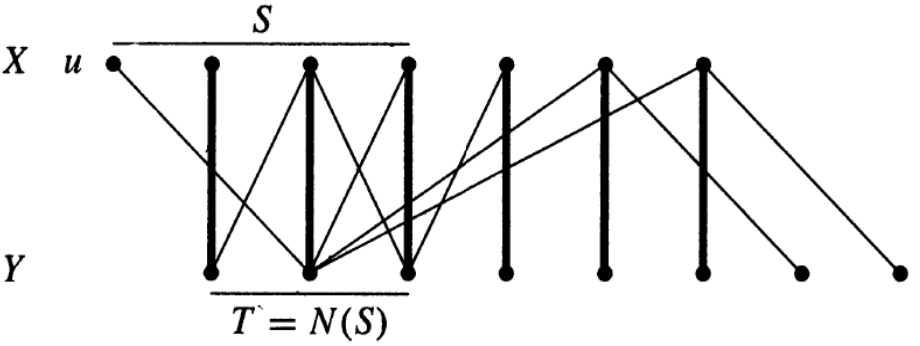
\includegraphics[width=.6\textwidth]{mat-hall-matching}
  \caption{Choose $S \subseteq X$ from an $X, Y$-bigraph $G$. $T = N(S) \subseteq Y$ is the neighbors of $S$. $u \in S$.}
  \label{fig:mat-hall-matching}
\end{figure}

\textbf{Proof} of \cref{thm:mat-hall-matching}: To prove $Q \implies P$ ($\neg P \implies \neg Q$):

\begin{enumerate}
  \item We use the contrapositive method with more efforts.

    \begin{supplement}
      \item $\neg P \implies \neg Q$ means if there is a maximum matching $M$ in an $X, Y$-bigraph $G$, and $M$ cannot saturate $X$, then $\abs{N(S)} < \abs{S}$.

      \item Here we utilize a maximum matching $M$, for if $M$ cannot saturate $X$, then it's much more impossible for the other matchings to saturate $X$.

      \item If $M$ is a maximum matching in $G$ and $M$ does not saturate $X$, then we obtain a set $S \subseteq X$ such that $\abs{N(S)} < \abs{S}$.
    \end{supplement}

  \item Let $u \in X$ be a vertex unsaturated by $M$.

  \item Among all the vertices reachable from $u$ by $M$-alternating paths in $G$, let $S$ consist of those in $X$, and let $T$ consist of those in $Y$ (see \cref{fig:mat-hall-matching} with $M$ in bold). Note that $u \in S$.

  \item We claim that $M$ matches $T$ with $S-\{u\}$. The $M$-alternating paths from $u$ reach $Y$ along edges not in $M$ and return to $X$ along edges in $M$. Hence every vertex of $S-\{u\}$ is reached by an edge in $M$ from a vertex in $T$. Since there is no $M$-augmenting path, every vertex of $T$ is saturated; thus an $M$-alternating path reaching $y \in T$ extends via $M$ to a vertex of $S$. Hence these edges of $M$ yield a bijection from $T$ to $S-\{u\}$, and we have $|T|=|S-\{u\}|$.

  \item The matching between $T$ and $S - \{u\}$ yields $T \subseteq N(S)$. In fact, $T = N(S)$. Suppose that $y \in Y-T$ has a neighbor $v \in S$. The edge $v y$ cannot be in $M$, since $u$ is unsaturated and the rest of $S$ is matched to $T$ by $M$. Thus adding $v y$ to an $M$-alternating path reaching $v$ yields an $M$-alternating path to $y$. This contradicts $y \notin T$, and hence vy cannot exist.

  \item With $T = N(S)$, we have proved that $\abs{N(S)} = \abs{T} = \abs{S} - 1 < \abs{S}$ for this choice of $S$. This completes the proof of the contrapositive.
\end{enumerate}

The proofs of \cref{thm:mat-hall-matching} are important.

\recall[\sectionprefix]{con-regular-bipartite-graph}

\begin{proposition}{}{mat-regular-perfect-matching}
  (3.1.13. Corollary in text)
  For $k>0$, every $k$-regular bipartite graph has a perfect matching.
\end{proposition}

\textbf{Proof} of \cref{prop:mat-regular-perfect-matching}:
\begin{enumerate}
  \item Let $G$ be a $k$-regular $X, Y$-bigraph. Counting the edges by endpoints in $X$ and by endpoints in $Y$ shows that $k \abs{X} = k \abs{Y}$, so $\abs{X} = \abs{Y}$. Hence it suffices to verify Hall's Condition; a matching that saturates $X$ will also saturate $Y$ and be a perfect matching.

  \item Consider $S \subseteq X$. Let $m$ be the number of edges from $S$ to $N(S)$. Since $G$ is $k$-regular, $m = k \abs{S}$. These $m$ edges are incident to $N(S)$, so $m \leq k \abs{N(S)}$. Hence $k \abs{S} \leq k \abs{N(S)}$, which yields $\abs{N(S)} \geq \abs{S}$ when $k>0$. Having chosen $S \subseteq X$ arbitrarily, we have established Hall's condition.
\end{enumerate}

\begin{definition}{}{mat-vertex-cover}
  (3.1.14. Definition in text)
  A \textbf{vertex cover} of a graph $G$ is a set $Q \subseteq V(G)$ that contains at least one endpoint of every edge. The vertices in $Q$ \textbf{cover} $E(G)$.
\end{definition}

Finding the minimum vertex cover is an NP-complete problem.

Since no vertex can cover two edges of a matching $M$, the size of every vertex cover $Q$ is at least the size of every matching ($\abs{M} \leq \abs{Q}$). Therefore, \textbf{obtaining a matching and a vertex cover of the same size PROVES that each is optimal}. Such proofs exist for bipartite graphs, but not for all graphs. "$M$ and $Q$ are optimal" refers that if $\abs{M} = \abs{Q}$, then $M$ is a maximum matching in $G$, and $Q$ is the minimum vertex cover in $G$.

\begin{figure}[htbp]
  \centering
  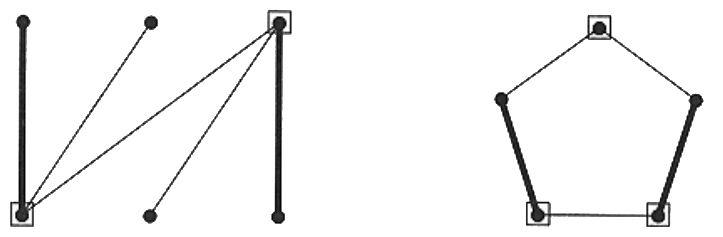
\includegraphics[width=.5\textwidth]{mat-vertex-cover}
  \caption{(3.1.15. Example in text)In the two graphs, bold edges are edges in a matching $M$, while rectangle highlighted vertices form a vertex cover $Q$. In the left graph, since $|M| = |Q|$, both $M$ and $Q$ are optimal. In the right graph, since $|M| < |Q|$, one or both is not optimal.}
  \label{fig:mat-vertex-cover}
\end{figure}

\textbf{Proof} of "if for a matching $M$ and a vertex cover $Q$ in a bigraph $G$, if $\abs{M} = \abs{Q}$, then then $M$ is a maximum matching in $G$, and $Q$ is the minimum vertex cover in $G$:

\begin{enumerate}
  \item We prove it by contradiction.
  \item Suppose when $\abs{M} = \abs{Q}$, $M$ and $Q$ are not optimal. There are two cases:

  \item Case 1: $M$ is not a maximum matching:
    \begin{enumerate*}
      \item Let $M'$ be a maximum matching, and $\abs{M'} > \abs{M}$.
      \item Since $\abs{M} = \abs{Q}$, we have $\abs{M'} > \abs{Q}$.
      \item By \cref{def:mat-vertex-cover}, $\abs{M'} \leq \abs{Q}$. As a result, the assumption is wrong.
    \end{enumerate*}

  \item Case 2: $Q$ is not a minimum vertex cover:
    \begin{enumerate*}
      \item Let $Q'$ be the minimum vertex cover, and $\abs{Q'} < \abs{Q} = \abs{M}$.
      \item Similarly, sine it contradicts to \cref{def:mat-vertex-cover}, the assumption is wrong.
    \end{enumerate*}
\end{enumerate}

\begin{theorem}{}{mat-bipartite-optimal-matching}
  (3.1.16. Theorem in text) (König [1931], Egerváry [1931])

  If $G$ is a bipartite graph, then the maximum size of a matching in $G$ equals the minimum size of a vertex cover of $G$. (Using notations defined in \cref{tab:mat-notations}, it means $\alpha'(G) = \beta(G)$.)
\end{theorem}

\textbf{Proof} of \cref{thm:mat-bipartite-optimal-matching}:

\begin{enumerate}
  \item Goal: Given the minimum vertex cover $Q$ exists, construct a matching $M$ of size $\abs{Q}$ exists. By $\abs{M} \leq \abs{Q}$, $M$ is a maximum matching.

  \item Let $G$ be an $X, Y$-bigraph. Since distinct vertices must be used to cover the edges of a matching, $|Q| \geq |M|$ whenever $Q$ is a vertex cover and $M$ is a matching in $G$. Given a smallest vertex cover $Q$ of $G$, we construct a matching of size $|Q|$ to prove that equality can always be achieved.

  \item Partition $Q$ by letting $R = Q \cap X$ and $T = Q \cap Y$ (since we know $V(G) = X \cap Y$). Let $H$ and $H'$ be the subgraphs of $G$ induced by $R \cup (Y - T)$ and $T \cup(X - R)$, respectively. We use Hall's Theorem to show that $H$ has a matching that saturates $R$ into $Y - T$ and $H'$ has a matching that saturates $T$. Since $H$ and $H'$ are disjoint, the two matchings together form a matching of size $|Q|$ in $G$.

  \item Since $R \cup T$ is a vertex cover, $G$ has no edge from $Y-T$ to $X-R$. For each $S \subseteq R$, we consider $N_H(S)$, which is contained in $Y-T$. (Proof by contradiction) If $\abs{N_H(S)} < \abs{S}$, then we can substitute $N_H(S)$ for $S$ in $Q$ to obtain a smaller vertex cover, since $N_H(S)$ covers all edges incident to $S$ that are not covered by $T$.

  \item The minimality of $Q$ thus yields Hall's Condition in $H$, and hence $H$ has a matching that saturates $R$. Applying the same argument to $H'$ yields the matching that saturates $T$.
\end{enumerate}

\subsubsection{Independent Sets and Covers}

\begin{definition}{}{mat-independence-number}
  The \textbf{independence number} of a graph is the maximum size of an independent set of vertices.
\end{definition}

Note: (3.1.18. Example in text) The independent number of a bipartite graph does not always equal the size of a partite set, but the size of the largest partite set is the lower bound. See \cref{fig:mat-independence-number}.

\begin{figure}[htbp]
  \centering
  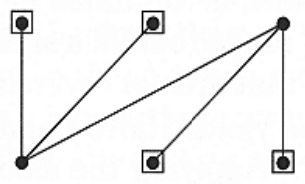
\includegraphics[width=.3\textwidth]{mat-independence-number}
  \caption{The independence number of this bipartite graph is 4 (rectangle highlighted vertices) rather than the intuitive 3.}
  \label{fig:mat-independence-number}
\end{figure}

\begin{definition}{}{mat-edge-cover}
  (3.1.19. Definition in text)
  An \textbf{edge cover} of $G$ is a set $L$ of edges such that every vertex of $G$ is incident to some edge of $L$.
\end{definition}

In \cref{fig:mat-independence-number}, the 4 edges connected to the independent set form an edge cover, but is not the minimum one.

\begin{table}[htbp]
  \centering
  \begin{tabular}{lll}
    \hline
    \textbf{Notation} & \textbf{Meaning}                & \textbf{Subset of vertices or edges} \\ \hline
    $\alpha(G)$       & Maximum size of independent set & Vertices                             \\
    $\alpha'(G)$      & Maximum size of matching        & Edges                                \\
    $\beta(G)$        & Minimum size of vertex cover    & Vertices                             \\
    $\beta'(G)$       & Minimum size of edge cover      & Edges                                \\ \hline
  \end{tabular}
  \caption{(3.1.20. Definition in text) Important and common notations for the optimal sizes of the sets in independence and covering problems.}
  \label{tab:mat-notations}
\end{table}

You must remember the four notations in \cref{tab:mat-notations} because these notations are commonly used in graph theory without an introduction, likewise for the questions in the exams.

\begin{lemma}{}{mat-independent-set-vertex-cover}
  (3.1.21. Lemma in text)
  In a graph $G$, $S \subseteq V(G)$ is an independent set iff $\bar{S}$ is a vertex cover, and hence $\alpha(G) + \beta(G) = n(G)$.
\end{lemma}

\textbf{Proof} of \cref{lem:mat-independent-set-vertex-cover}:
\begin{enumerate*}
  \item $S$ is an independent set.
  \item $\rightarrow$ Every edge is incident to \textbf{at least one} vertex in $\bar{S}$ (the complement of $S$).
  \item $\rightarrow$ $\bar{S}$ cover all edges.
  \item $\rightarrow$ No edges joining vertices of $S$.
  \item $\rightarrow$ Every maximum independent set is the complement of a minimum vertex cover.
\end{enumerate*}

Continuing from \cref{lem:mat-independent-set-vertex-cover}, $S$ is a maximum independent set iff. $\bar S$ is the minimum vertex cover.

\begin{figure}[htbp]
  \centering
  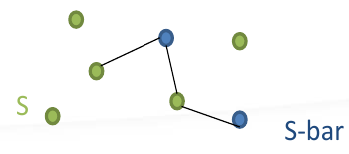
\includegraphics[width=.4\textwidth]{mat-independent-set-vertex-cover}
  \caption{In this graph $G$, }
  \label{fig:mat-independent-set-vertex-cover}
\end{figure}

\begin{theorem}{}{mat-isolated-vertices}
  (3.1.22. Theorem in text)
  \def\abst#1{\ensuremath{\abs{\text{#1}}}}%
  If $G$ is a graph without isolated vertices, then $\alpha'(G) + \beta(G') = n(G)$.

  (\abst{Maximum matching} + \abst{Minimum edge cover} = \abst{All vertices})
\end{theorem}

\textbf{Proof} of \cref{thm:mat-isolated-vertices} in the textbook:

\begin{enumerate}
  \item From a maximum matching $M$, we will construct an edge cover of size $n(G) - \abs{M}$. Since a smallest edge cover is no bigger than this cover, this will imply that $\beta'(G) \leq n(G) - \alpha'(G)$.'

    \begin{supplement}
      Given a maximum matching $M$, construct an edge cover of size

      $n(G)-|M| \Rightarrow \beta'(G) \leq n(G)-\alpha'(G)$
    \end{supplement}

  \item Also, from a minimum edge cover $L$, we will construct a matching of size $n(G) - \abs{L}$. Since a largest matching is no smaller than this matching, this will imply that $\alpha'(G) \geq n(G) - \beta'(G)$. These two inequalities complete the proof.

    \begin{supplement}
      Adding to $M$ one edge incident to each unsaturated vertex

      $\therefore \text { total size of this edge cover }=n(G)-2|M|+|M|=n(G)-|M|$

    \end{supplement}

  \item Let $M$ be a maximum matching in $G$. We construct an edge cover of $G$ by adding to $M$ one edge incident to each unsaturated vertex. We have used one edge for each vertex, except that each edge of $M$ takes care of two vertices, so the total size of this edge cover is $n(G) - \abs{M}$, as desired.

  \item Now let $L$ be a minimum edge cover. If both endpoints of an edge $e$ belong to edges in $L$ other than $e$, then $e \notin L$, since $L - \{e\}$ is also an edge cover. Hence each component formed by edges of $L$ has at most one vertex of degree exceeding 1 and is a star (a tree with at most one non-leaf). Let $k$ be the number of these components. Since $L$ has one edge for each non-central vertex in each star, we have $\abs{L} = n(G) - k$. We form a matching $M$ of size $k = n(G) - \abs{L}$ by choosing one edge from each star in $L$.

    \begin{supplement}
      Given a minimum edge cover $L$, construct a matching of size

      $n(G)-|L| \Rightarrow \alpha'(G) \geq n(G)-\beta'(G)$

      Each component formed by edges of $L$ is a star $k$ : the number of these components

      $\therefore|L|=n(G)-k$

      Choosing one edge from each star in $L$ form a matching of size $k=n(G)-|L|$

      $\because n(G) \geq \beta'(G)+\alpha'(G) \text { and } n(G) \leq \alpha'(G)+\beta'(G)^{\mathfrak{I}}$

      $\therefore n(G)=\alpha'(G)+\beta'(G)$
    \end{supplement}
\end{enumerate}

\textbf{Proof} of \cref{thm:mat-isolated-vertices} arranged by the instructor:

\begin{enumerate}
  \def\abst#1{\ensuremath{\abs{\text{#1}}}}%
  \item Idea 1: Given a maximum matching $M$, we want to create an edge cover $L$ such that $\abs{L} = n(G) + \abs{M}$, where $\abs{M} = \alpha'(G)$.

  \item If $L$ exists, $\beta'(G) \leq n(G) - \alpha'(G)$ \\
    (\abst{Minimum edge cover} $\leq$ \abst{All vertices} - \abst{Maximum matching}) because $\beta'(G) \leq \abs{L}$.

  \item The following steps form an edge cover $L$ from a maximum matching $M$ of size 2 (black edges) in the graph $G$ shown in \cref{fig:mat-isolated-vertices-1}, where $G$ is a graph without isolated vertices.

  \item Let $L = M$. In this way, edges in $L$ covers their endpoints (blue vertices).

  \item To cover unsaturated vertices (orange vertices), there is no isolated vertex in $G$, there must be edges cover the currently unsaturated vertices, but such edges are not in the matching $M$ to avoid a shared vertex in $M$.

  \item Since we don't care shared vertices in an edge cover, we can add an edge in $G$ to $L$ to connect any vertex in $L$ to each of unsaturated vertices, saying these edges are red ones.

  \item Since $L$ saturates all vertices, $L$ is an edge cover (with 2 black and 2 red edges) of size \\
    $n(G) - 2 \abs{M} + \abs{M}$.

  \item The edge cover $L$ is a subset of edges of size $n(G) - \abs{M}$ because $L$ contains the following edges:
    \begin{enumerate*}
      \item All edges in $M$ (of size $\abs{M}$). For each edge in $M$, it covers two vertices. With all edges in $M$, there are $n(G) - 2 \abs{M}$ unsaturated vertices.
      \item An additional edge other than those in $M$ for each vertex unsaturated by edges in $M$. The number of these additional edges equals to $n(G) - 2 \abs{M}$.
    \end{enumerate*}

  \item In brief, what we can confirm now is that the edge cover $L$ constructed with the maximum matching $M$ is of size $\abs{L} = n(G) - \abs{M}$.

  \item Such edge cover $L$ is not necessary the minimum one (of size $\beta'(G)$), but it must not be smaller than the minimum one. That is:

    \begin{equation}
      \abs{L} = n(G) - \abs{M} \geq \beta'(G)
      \label{eq:mat-isolated-vertices-1}
    \end{equation}

  \item Since $M$ is a maximum matching (of size $\abs{M} = \alpha'(G)$), \cref{eq:mat-isolated-vertices-1} is equivalent to\\
    $n(G) - \alpha'(G) \geq \beta'(G)$. That is:

    \begin{equation}
      \alpha'(G) + \beta'(G) \leq n(G)
      \label{eq:mat-isolated-vertices-2}
    \end{equation}

  \item We want the other inequality with $\geq$ sign to make \cref{eq:mat-isolated-vertices-2} equality.

  \item Idea 2: Given a minimum edge cover $L$ (the other edge cover other than the above-mentioned $L$) of size $\abs{L} = \beta'{G}$, we want to construct a matching $M$ of size $n(G) - \abs{L}$. By definition, the size of $M$ must be at most the size of a maximum matching. That is, $\abs{M} = n(G) - \abs{L} \leq \alpha'(G)$. With $\abs{L} = \beta'{G}$, we have $n(G) - \beta'(G) \leq \alpha'(G)$ or equivalently, $\alpha'(G) \beta'(G) \geq n(G)$.

  \item The following steps construct such a matching $M$ from a given minimum edge cover $L$.

  \item $L$ is a minium edge cover. It means that $L$ contains all the edges required to cover all vertices.

  \item In $L$, will there be a path of size 3 ($P_4$)? It refers to the graph with arbitrary three edges isomorphic to an $N$-like path. The answer is no. As illustrated in \cref{fig:mat-isolated-vertices-2}, if there is a $P_4$, the center edge (orange one) is redundant in a minimum edge cover to cover the 4 vertices in a $P_4$.

  \item When will a $P_4$ exist in a bipartite graph? For example, all solid (bold and normal) edges in \cref{fig:mat-isolated-vertices-3} form a minimum edge cover $L$. In $L$, the maximum possible length of a path is 2 ($P_3$), so the author of this textbook calls this graph "a graph of stars", where a star refers to a component. For example, the 4 stars in \cref{fig:mat-isolated-vertices-4}.

  \item How to construct a matching $M$ from $k$ stars in a minimum edge cover $L$? Starting from an empty matching $M$, we can choose at most a single edge from each of $k$ stars to add the edge to the matching $M$. With any two edges from the same star, they must share at least a vertex. With $k$ stars, $\abs{M} = k$.

  \item The number of edges in the minimum edge cover $L$ is $\abs{L} = n(G) - k$, which we can calculate as follows:
    \begin{enumerate}
      \item Let the root be the center of each star. ("Center" of a star is defined by any single vertex with the maximum degree in the star. For a single node as a star, itself is the root.)
      \item For each star, every leaf can reach the root with a single edge. With $k$ stars, there are $k$ roots and $n(G) - k$ leaves. (The minimum edge cover $L$ covers all vertices.) By $n(G) - k$ leaves and an edge for each leaf, there are $n(G) - k$ edges. That is, $\abs{L} = n(G) - k$.
    \end{enumerate}

  \item By the definition and the number of edges in $\abs{L}$, we have $\abs{L} = \beta'(G) = n(G) - k$. That is:

    \begin{equation}
      k = n(G) - \beta'(G)
      \label{eq:mat-isolated-vertices-3}
    \end{equation}

  \item As a result, given a minimum edge cover $L$ of size $\abs{L} = \beta'(G)$, we can find a matching $M$ of size $\abs{M} = k = n(G) - \beta'(G)$. By definition, the size of $M$ cannot be larger than that of a maximum matching (of size $\alpha'(G)$). That is:

    \begin{equation}
      n(G) - \beta'(G) \leq \alpha'(G)
      \label{eq:mat-isolated-vertices-4}
    \end{equation}

    or equivalently,

    \begin{equation}
      \alpha'(G) + \beta'(G) \geq n(G)
      \label{eq:mat-isolated-vertices-5}
    \end{equation}

  \item By the two inequalities \cref{eq:mat-isolated-vertices-2,eq:mat-isolated-vertices-5}, we conclude that:

    \begin{equation}
      \alpha'(G) + \beta'(G) = n(G)
      \label{eq:mat-isolated-vertices-56}
    \end{equation}

\end{enumerate}

\begin{figure}
  \centering
  \begin{subfigure}[t]{.45\textwidth}
    \centering
    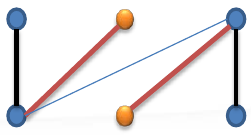
\includegraphics[width=.7\textwidth]{mat-isolated-vertices-1}
    \caption{The black edges form a maximum matching $M$ but leave orange vertices unsaturated.}
    \label{fig:mat-isolated-vertices-1}
  \end{subfigure}
  \hfill
  \begin{subfigure}[t]{.45\textwidth}
    \centering
    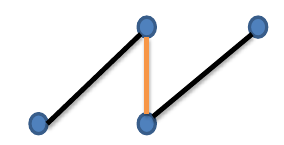
\includegraphics[width=.7\textwidth]{mat-isolated-vertices-2}
    \caption{An $N$-like path in a bipartite graph.}
    \label{fig:mat-isolated-vertices-2}
  \end{subfigure}

  \begin{subfigure}[t]{.45\textwidth}
    \centering
    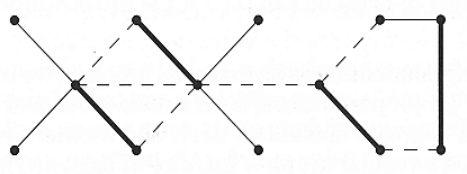
\includegraphics[width=.9\textwidth]{mat-isolated-vertices-3}
    \caption{The solid edges form a minimum edge cover $L$.}
    \label{fig:mat-isolated-vertices-3}
  \end{subfigure}
  \hfill
  \begin{subfigure}[t]{.45\textwidth}
    \centering
    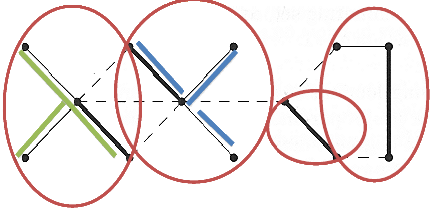
\includegraphics[width=.7\textwidth]{mat-isolated-vertices-4}
    \caption{There are 4 stars in the minimum edge cover $L$ of solid lines from left to right: (1) One with green edges, (2) another with blue edges, (3) yet another with a single edge, and (4) the other with two edges.}
    \label{fig:mat-isolated-vertices-4}
  \end{subfigure}

  \caption{The graphs to illustrate the proof of \cref{thm:mat-isolated-vertices}.}
  \label{fig:mat-isolated-vertices}
\end{figure}

\begin{corollary}{}{mat-isolated-vertices}
  If $G$ is a bipartite graph with no isolated vertices, than $\alpha(G) = \beta'(G)$.
\end{corollary}

\textbf{Proof} of \cref{cor:mat-isolated-vertices}:

\begin{enumerate*}
  \item By \cref{lem:mat-independent-set-vertex-cover,thm:mat-isolated-vertices}, we have
    $n(G) = \alpha(G) + \beta(G) = \alpha'(G) + \beta'(G)$

  \item By \cref{thm:mat-bipartite-optimal-matching}, we have
    $\alpha'(G) = \beta(G)$.

  \item Therefore, $\alpha(G) = \beta'(G)$.
\end{enumerate*}

\subsubsection{Dominating Sets}

\begin{definition}{}{mat-dominating-set}
  In a graph $G$, a set $S \subseteq V(G)$ is a \textbf{dominating set} if every vertex not in $S$ has a neighbor in $S$.

  The dominating number $\gamma(G)$ is the minimum size of a dominating set in $G$.
\end{definition}

Note that a dominating set refers to a vertex set dominating the other vertices through edges. See \cref{fig:mat-dominating-set} for an example.

\begin{figure}
  \centering
  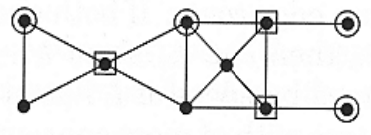
\includegraphics[width=.5\textwidth]{mat-dominating-set}
  \caption{(3.1.27. Example in text) This graph $G$ has a \textbf{minimal} dominating set of size 4 (circles) and a \textbf{minimum} dominating set of size 3 (squares): $\gamma(G)=3$.}
  \label{fig:mat-dominating-set}
\end{figure}

\begin{remark}{}{mat-dominating-set}
  When a graph $G$ has no isolated vertices, every vertex cover is a dominating set, so $\gamma(G) \leq \beta(G)$ (minimum size of a dominating set in $G$ is at most the size of the minimum vertex cover).

  To show the statement above, for a $K_n$ as shown in \cref{fig:mat-dominating-set-k4} ($K_4$), $\gamma \left( K_n \right) = 1$, and $\beta \left( K_n \right) = n - 1$.

  Every dominating set in a $k$-regular graph $G$ has size at least $\frac{n(G)}{k + 1}$.
\end{remark}

\begin{figure}[htbp]
  \centering
  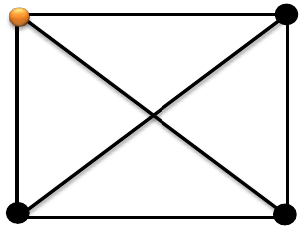
\includegraphics[width=.2\textwidth]{mat-dominating-set-k4}
  \caption{In a $K_4$, the dominating set can be the orange vertex.}
  \label{fig:mat-dominating-set-k4}
\end{figure}

\subsection{Algorithms and Applications}

\subsubsection{Maximum Bipartite Matching}

\begin{algorithm}{Augmenting Path Algorithm}{mat-augmenting-path}
  (3.2.1. Algorithm in text)

  \textbf{Input}: An $X, Y$-bigraph $G$, a matching $M$ in $G$, and the set $U$ of $M$-unsaturated vertices in $X$.

  \textbf{Idea}: Explore $M$-alternating paths from $U$, letting $S \subseteq X$ and $T \subseteq Y$ be the sets of vertices reached. Mark vertices of $S$ that have been explored for path extensions. As a vertex is reached, record the vertex from which it is reached.

  \textbf{Initialization}: $S=U$ and $T=\emptyset$.

  \textbf{Iteration}: If $S$ has no unmarked vertex, stop and report $T \cup(X-S)$ as a minimum cover and $M$ as a maximum matching. Otherwise, select an unmarked $x \in S$. To explore $x$, consider each $y \in N(x)$ such that $x y \notin M$. If $y$ is unsaturated, terminate and report an $M$-augmenting path from $U$ to $y$. Otherwise, $y$ is matched to some $w \in X$ by $M$. In this case, include $y$ in $T$ (reached from $x$ ) and include $w$ in $S$ (reached from $y$ ). After exploring all such edges incident to $x$, mark $x$ and iterate.
\end{algorithm}

\begin{remark}{}{mat-augmenting-path}
  (3.2.4 Remark in text)
  The time complexity of \cref{alg:mat-augmenting-path} is $O(n m)$ for a bigraph with $n$ vertices and $m$ edges.

  Theorem 3.2.22 in the textbook provides an $O(\sqrt{n} m)$-time algorithm (Hopcroft-Karp [1973]), while in Section 3.3 in the textbook, there is an $O(\sqrt{n} m)$-time algorithm for more general problems (Even and Tarjan [1975]).
\end{remark}

\begin{figure}
  % NOTE: for a larger figure, you may want to split sub-figures into pages with \ContinuedFloat
  % reference: https://tex.stackexchange.com/a/278748
  \def\width{.3\textwidth}%
  \def\gap{\hspace{.04\textwidth}}%
  \centering
  \begin{subfigure}[t]{\width}
    \centering
    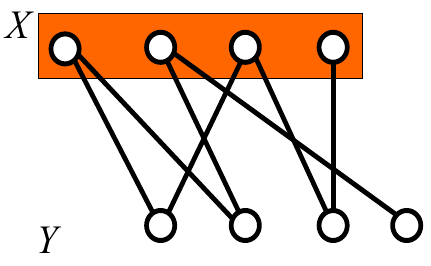
\includegraphics[width=.9\textwidth]{mat-aug-0}
    \caption{The initial state: $S = U = X$ (vertices in the orange rectangle) and $T = \emptyset$.}
    \label{fig:mat-aug-0}
  \end{subfigure}
  \gap
  \begin{subfigure}[t]{\width}
    \centering
    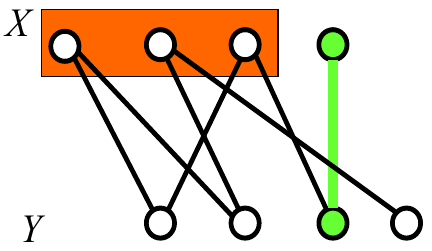
\includegraphics[width=.9\textwidth]{mat-aug-1}
    \caption{Iteration 1: Select an unmarked (white) $x \in S$, saying the rightmost one. $\exists y \in N(x)$, so report $xy$, saturate $y$ with $xy$ (include $xy$ in $M$), and mark $x$.}
    \label{fig:mat-aug-1}
  \end{subfigure}
  \gap
  \begin{subfigure}[t]{\width}
    \centering
    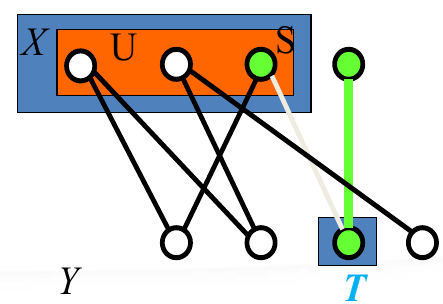
\includegraphics[width=.8\textwidth]{mat-aug-2}
    \caption{Iteration 2-1: For $x \in S$, saying the rightmost one, through the white edge, the green $y \in N(x)$ is saturated by $wy$ ($w \in X$), so add $y$ to $T$, add $w$ back to $S$, and make $xy$ dashed.}
    \label{fig:mat-aug-2-1}
  \end{subfigure}

  \begin{subfigure}[t]{\width}
    \centering
    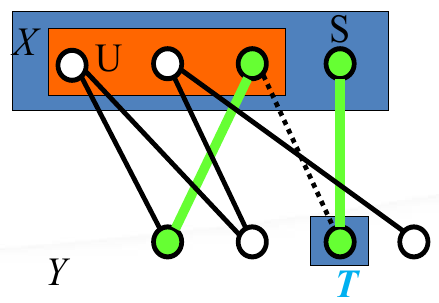
\includegraphics[width=.7\textwidth]{mat-aug-3}
    \caption{Iteration 2-2: With the previous $x$, through the green edge, since the left green $y \in N(x)$ is unsaturated, report $xy$, saturate $y$ with $xy$ (include $xy$ in $M$), mark $x$ and $w$, and reset $T$ to $\emptyset$.}
    \label{fig:mat-aug-2-2}
  \end{subfigure}
  \gap
  \begin{subfigure}[t]{\width}
    \centering
    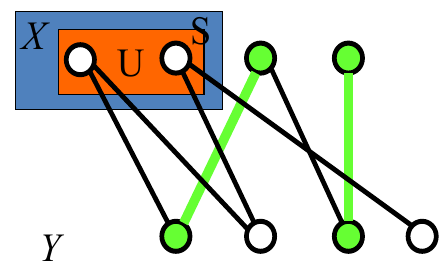
\includegraphics[width=.8\textwidth]{mat-aug-4}
    \caption{Iteration 3-0: Before iteration 3.}
    \label{fig:mat-aug-3-0}
  \end{subfigure}
  \gap
  \begin{subfigure}[t]{\width}
    \centering
    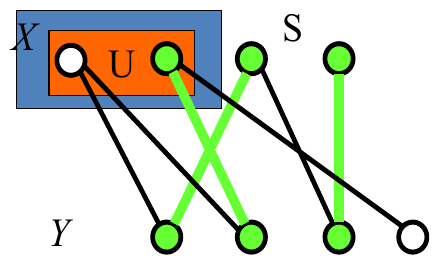
\includegraphics[width=.8\textwidth]{mat-aug-5}
    \caption{Iteration 3-1: For the rightmost $x \in S$, through the green edge, $y \in N(x)$ is unsaturated, so report $xy$, saturate $y$ with $xy$, and mark $x$}
    \label{fig:mat-aug-3-1}
  \end{subfigure}

  \begin{subfigure}[t]{\width}
    \centering
    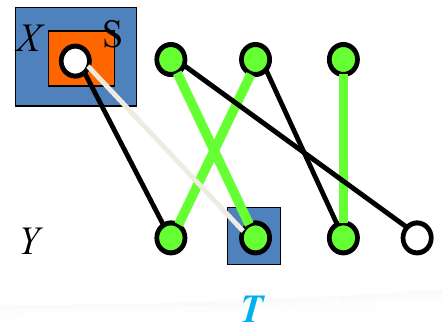
\includegraphics[width=.9\textwidth]{mat-aug-6}
    \caption{Iteration 4-1: For the rightmost $x \in S$, through the white edge, $y \in N(x)$ is saturated by $wy$ $w \in X$, so add $y$ to $T$, add $w$ back to $S$, and make $xy$ dashed.}
    \label{fig:mat-aug-4-1}
  \end{subfigure}
  \gap
  \begin{subfigure}[t]{\width}
    \centering
    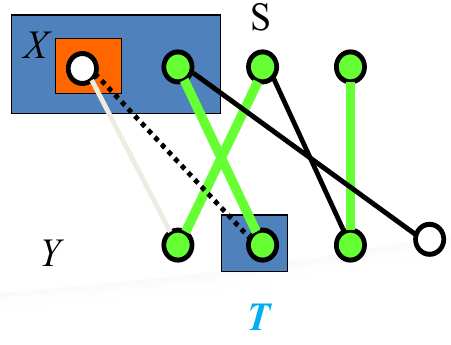
\includegraphics[width=.9\textwidth]{mat-aug-7}
    \caption{Iteration 4-2: Repeat iteration 4-1 but with the other $y \in N(x)$.}
    \label{fig:mat-aug-4-2}
  \end{subfigure}
  \gap
  \begin{subfigure}[t]{\width}
    \centering
    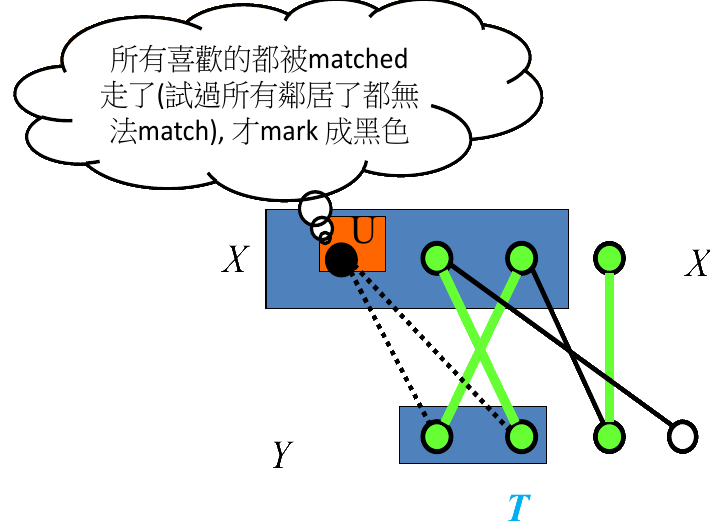
\includegraphics[width=\textwidth]{mat-aug-8}
    \caption{Iteration 4-3: Since every $y \in N(x)$ is saturated, mark $x$ black.}
    \label{fig:mat-aug-4-3}
  \end{subfigure}

  \begin{subfigure}[t]{\width}
    \centering
    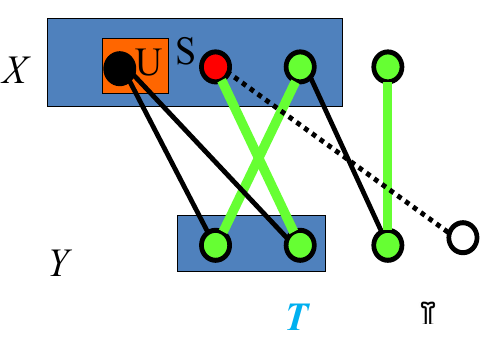
\includegraphics[width=.9\textwidth]{mat-aug-9}
    \caption{Iteration 4-4: For some $t \in T$, saying the rightmost one, we observe that the red $w \in N(t)$ has an unsaturated neighbor $y \in Y$ through $wy$ (the dashed edge).}
    \label{fig:mat-aug-4-4}
  \end{subfigure}
  \gap
  \begin{subfigure}[t]{\width}
    \centering
    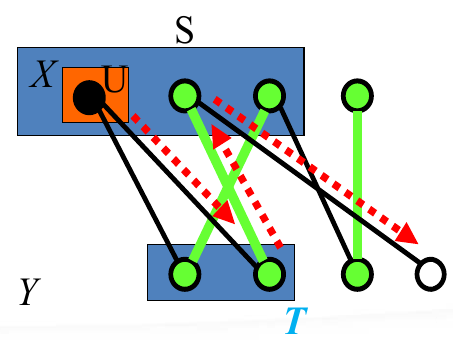
\includegraphics[width=.9\textwidth]{mat-aug-10}
    \caption{Iteration 4-5: By remove $wt$ in $M$, but report $wy$ and $xt$, we can mark $x$ green, and clear $S$.}
    \label{fig:mat-aug-4-5}
  \end{subfigure}
  \gap
  \begin{subfigure}[t]{\width}
    \centering
    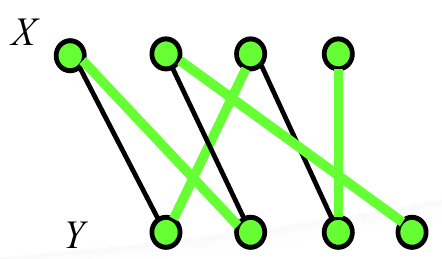
\includegraphics[width=\textwidth]{mat-aug-11}
    \caption{Iteration 5: Since $S$ has not unmarked vertex ($U = \emptyset$), the green edges form a maximum matching.}
    \label{fig:mat-aug-5}
  \end{subfigure}

  \caption{The process of \cref{alg:mat-augmenting-path} given an $X, Y$-bigraph $G$ with an empty matching $M$ as shown in \cref{fig:mat-aug-0}.}
  \label{fig:mat-aug}
\end{figure}

In the exams, you may be asked to find a maximum matching with the augmenting path algorithm (\cref{alg:mat-augmenting-path}) given a bipartite graph.

\end{document}